% Standalone TikZ figure: Technology Evolution Timeline
% For Chapter 10: Conclusion and Future Directions
\documentclass[tikz,border=10pt]{standalone}
\usepackage{tikz}
\usetikzlibrary{arrows.meta, positioning, shapes.geometric, calc, decorations.pathmorphing}

\begin{document}
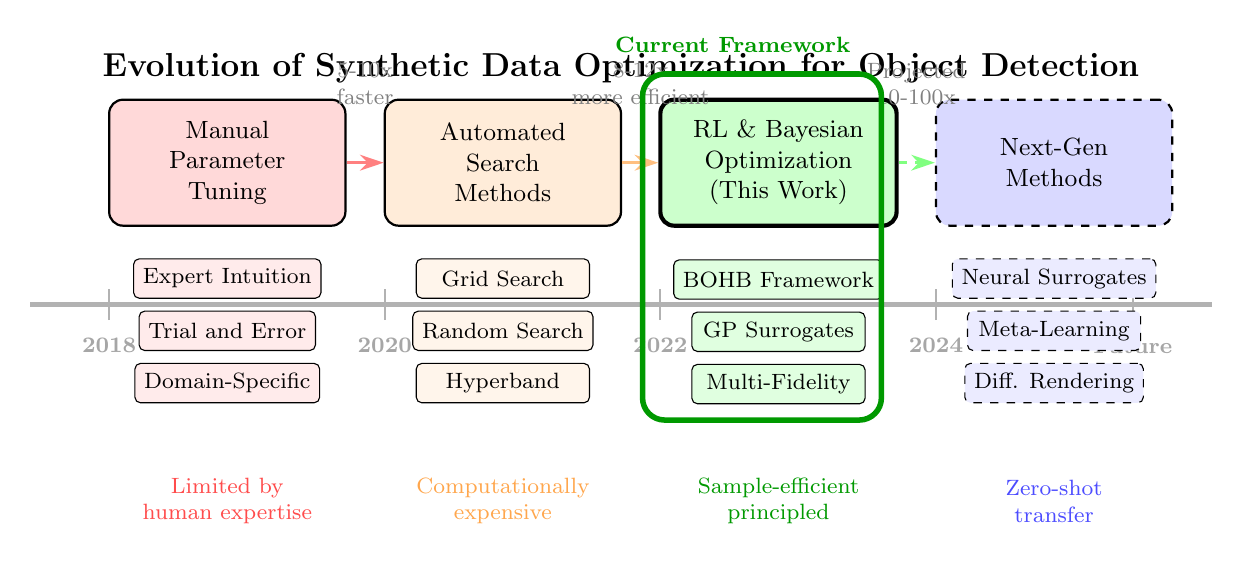
\begin{tikzpicture}[
    node distance=0.8cm,
    every node/.style={font=\small},
    era/.style={rectangle, draw, thick, minimum width=3cm, minimum height=1.6cm, align=center, rounded corners=5pt},
    feature/.style={rectangle, draw, minimum width=2.2cm, minimum height=0.5cm, align=center, rounded corners=2pt, font=\footnotesize},
    arrow/.style={-{Stealth[length=3mm, width=2mm]}, very thick},
    timeline/.style={line width=2pt},
    title/.style={font=\bfseries\large}
]

% Title
\node[title] at (6.5, 3) {Evolution of Synthetic Data Optimization for Object Detection};

% Timeline axis
\draw[timeline, gray!60] (-1, 0) -- (14, 0);

% Era markers on timeline
\foreach \x/\year in {0/2018, 3.5/2020, 7/2022, 10.5/2024, 13/Future} {
    \draw[thick, gray!60] (\x, -0.2) -- (\x, 0.2);
    \node[below, font=\footnotesize\bfseries, gray!70] at (\x, -0.3) {\year};
}

% ============ ERA 1: Manual Tuning ============
\node[era, fill=red!15] (era1) at (1.5, 1.8) {Manual\\Parameter\\Tuning};
\node[feature, fill=red!8, below=0.4cm of era1] (f1a) {Expert Intuition};
\node[feature, fill=red!8, below=0.15cm of f1a] (f1b) {Trial and Error};
\node[feature, fill=red!8, below=0.15cm of f1b] (f1c) {Domain-Specific};

% ============ ERA 2: Grid/Random Search ============
\node[era, fill=orange!15] (era2) at (5, 1.8) {Automated\\Search\\Methods};
\node[feature, fill=orange!8, below=0.4cm of era2] (f2a) {Grid Search};
\node[feature, fill=orange!8, below=0.15cm of f2a] (f2b) {Random Search};
\node[feature, fill=orange!8, below=0.15cm of f2b] (f2c) {Hyperband};

% ============ ERA 3: Current Framework (BO/RL) ============
\node[era, fill=green!20, line width=1.5pt] (era3) at (8.5, 1.8) {RL \& Bayesian\\Optimization\\(This Work)};
\node[feature, fill=green!12, below=0.4cm of era3] (f3a) {BOHB Framework};
\node[feature, fill=green!12, below=0.15cm of f3a] (f3b) {GP Surrogates};
\node[feature, fill=green!12, below=0.15cm of f3b] (f3c) {Multi-Fidelity};

% ============ ERA 4: Future ============
\node[era, fill=blue!15, dashed] (era4) at (12, 1.8) {Next-Gen\\Methods};
\node[feature, fill=blue!8, below=0.4cm of era4, dashed] (f4a) {Neural Surrogates};
\node[feature, fill=blue!8, below=0.15cm of f4a, dashed] (f4b) {Meta-Learning};
\node[feature, fill=blue!8, below=0.15cm of f4b, dashed] (f4c) {Diff. Rendering};

% Arrows between eras
\draw[arrow, red!50] (era1.east) -- (era2.west);
\draw[arrow, orange!50] (era2.east) -- (era3.west);
\draw[arrow, green!50, dashed] (era3.east) -- (era4.west);

% Performance improvement indicators
\node[font=\footnotesize, text=gray, align=center] at (3.25, 2.8) {5-10x\\faster};
\node[font=\footnotesize, text=gray, align=center] at (6.75, 2.8) {8-12x\\more efficient};
\node[font=\footnotesize, text=gray, align=center] at (10.25, 2.8) {Projected\\10-100x};

% Bottom annotations
\node[font=\footnotesize, text=red!70, align=center] at (1.5, -2.5) {Limited by\\human expertise};
\node[font=\footnotesize, text=orange!70, align=center] at (5, -2.5) {Computationally\\expensive};
\node[font=\footnotesize, text=green!60!black, align=center] at (8.5, -2.5) {Sample-efficient\\principled};
\node[font=\footnotesize, text=blue!70, align=center] at (12, -2.5) {Zero-shot\\transfer};

% Highlight current work
\draw[line width=2pt, green!60!black, rounded corners=8pt]
    ([shift={(-0.2,0.3)}]era3.north west) rectangle ([shift={(0.2,-0.2)}]f3c.south east);
\node[font=\footnotesize\bfseries, text=green!60!black, anchor=west] at (6.3, 3.3) {Current Framework};

\end{tikzpicture}
\end{document}
